% !TEX TS-program = pdflatex
% !TEX encoding = UTF-8 Unicode

\documentclass[a4paper]{article}

\usepackage[swedish]{babel}
\usepackage[T1]{fontenc}
\usepackage[utf8]{inputenc}
\usepackage[pdftex]{graphicx}
\usepackage{float}
\usepackage{fancyhdr}
\usepackage[toc,page]{appendix}
\usepackage{listings}
\usepackage{booktabs} % for much better looking tables
\usepackage{array} % for better arrays (eg matrices) in maths
\usepackage{paralist} % very flexible & customisable lists (eg. enumerate/itemize, etc.)
\usepackage{verbatim} % adds environment for commenting out blocks of text & for better verbatim
\usepackage{subfig} % make it possible to include more than one captioned figure/table in a single float

\def\changemargin#1#2{\list{}{\rightmargin#2\leftmargin#1}\item[]}
\let\endchangemargin=\endlist 

%%% HEADERS & FOOTERS
\author{Jonathan Karlsson, Niclas Olofsson, Paul Nedstrand\\jonka293, nicol, paune\\Grupp 2}
\pagestyle{fancy} % options: empty , plain , fancy
\renewcommand{\headrulewidth}{1pt} % customise the layout...
\fancyhead[LO,LE]{Jonathan, Niclas, Paul\\Rapport lab 2-3}
\lfoot{}\cfoot{\thepage}\rfoot{}

%%%% SECTION TITLE APPEARANCE
%\usepackage{sectsty}
%\allsectionsfont{\sffamily\mdseries\upshape} % (See the fntguide.pdf for font help)
%% (This matches ConTeXt defaults)
%
%%%% ToC (table of contents) APPEARANCE
%\usepackage[nottoc,notlof,notlot]{tocbibind} % Put the bibliography in the ToC
%\usepackage[titles,subfigure]{tocloft} % Alter the style of the Table of Contents
%\renewcommand{\cftsecfont}{\rmfamily\mdseries\upshape}
%\renewcommand{\cftsecpagefont}{\rmfamily\mdseries\upshape} % No bold!

%%% END Article customizations

%%% The "real" document content comes below...

\title{Rapport lab 2-3\\ \vspace{2 mm} {\large TSEA44}}
%\date{} % Activate to display a given date or no date (if empty),
         % otherwise the current date is printed 

\begin{document}
\maketitle

\newpage

\tableofcontents

\newpage
\section{Labb 2}
\subsection{Introduktion}
Syftet med denna laboration var att konstruera en accelerator för jpeg-komprimering från raw-filer, i hårdvara. Detta löstes med hjälp av programmeringsspråket system verilog och genom att bygga vidare på det existerande skelettet som gavs med uppgiften. I första delen (labb2) så har vi en dator som styr själva acceleratorn och skickar all data via en bus för att sedan behandlas och lagras i ett blockminne där datorn sedan får läsa av resultatet. Ett register används för att starta grunkan och sedan läsa av att resultatet finns att hämta.

Det jpeg-acceleratorn gör är att ta ett block med 8x8 pixlar, skicka in det i en givet DCT maskin som gör komprimeringar av pixlarna, sedan transponeras de 8x8 pixlarna i ett minne och skickas tillbaka till DCT\rq{}n för att gå igenom en gång till. Alla pixlar multipliceras nu med hårdkodade reciprokaler och läggs i ett utminne. 

Datorn kan nu läsa av minnet, transponera och spara ner till en jpeg fil som kan öppnas på vanligt sätt.

\subsection{Tillståndsgraf och arkitektur}
En vidare hjälp är att den DCT maskin som gör beräkningar är redan given så problemet som skall lösas innebär att skapa signaler för att styra DCT\rq{}n, ett blockminne för indata och ett för utdata, ett minne där vi transponerar samt en maskin som utför multiplikationerna med reciprokalerna.

\begin{figure}[h]
\centering
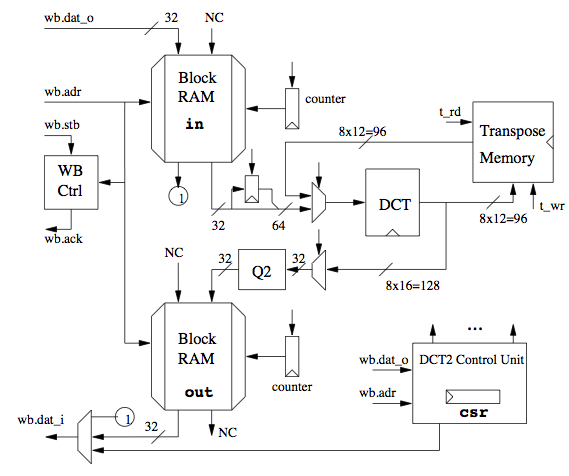
\includegraphics[scale=0.5]{architecture.png}
\caption{Arkitektur för vår design}
\label{fig:architecture}
\end{figure}

Figur \ref{fig:architecture} visar den arkitektur som konstruerades för att lösa uppgiften. All data som kommer in från bussen läggs in i minnet och vi väntar sedan på en startsignal från datorn. Då används räknaren tillsammans med en vippa för att skicka in data till DCT\rq{}n för att sedan skriva in 8x8 pixlar till transponeringsminnet, när vi skrivit klart där så läser vi av kolumnerna (och får därigenom transponeringen), skickar in till DCT\rq{}n igen.

Ett problem vi hade så här långt var klockningen, när vi skickar in data från inminnet så måste vi göra det 8 pixlar åt gången, men i minnet finns bara 4 pixlar per rad, så vi måste läsa två rader (därav vippan), vidare måste vi klocka ner DCT\rq{}n en klockcykel för att den ska \lq\lq{}hinna med\rq\rq{}. Läsningen från transponeringen var inget problem, däremot när pixlarna kommer ut den andra gången måste klockningen anpassas till Q2-maskinen då den tar två pixlar per klockcykel så DCT\rq{}n måste gå ytterligare långsammare för att detta ska fungera.

\begin{figure}[h]
\centering
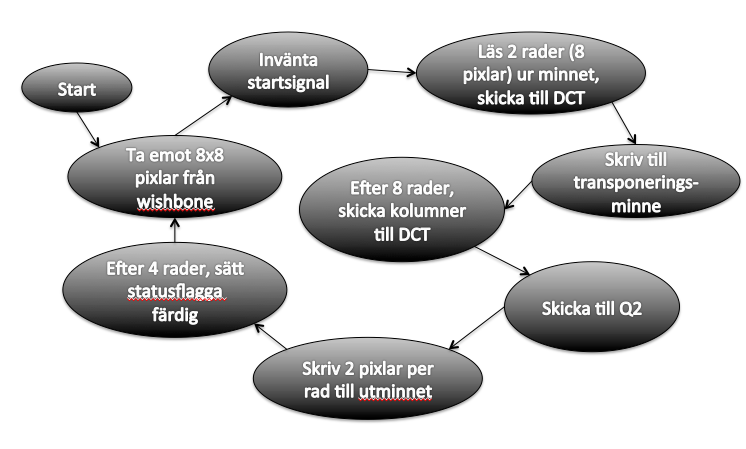
\includegraphics[width=340px]{states.png}
\caption{Tillståndsgraf för vår design}
\label{fig:state}
\end{figure}
Figur \ref{fig:state} visar en tillståndsgraf över maskinen och dess procedur för att komprimera raw-filer till jpeg. Tillståndsgrafen följer precis det schema som arkitekturen i figur \ref{fig:architecture} också visar.

\subsection{Vidare frågor man kan ställa sig}
\begin{itemize}
	\item Hur vi verifierade att vår DCT hårdvara fungerade korrekt?
\end{itemize}
Vi använde oss av matlab för att räkna ut ett antal exempel som vi kunde simulera i ModelSim, genom att jämföra vad matlab gav för resultat med det som låg i utminnet efter en simulering lyckades vi bekräfta att acceleratorn hade gjort sitt jobb.

\begin{itemize}
	\item Är storleken på DCT hårdvaran jämförbar med den förbättrade prestandan?
\end{itemize}
Hela grunkan tar upp en hel del hårdvara och på grund av att det är så mycket kommunikation, vi måste klocka DCT\rq{}n annorlunda och att Q2 är så långsam så är det frågan om det verkligen är värt det. I de kommande laborationerna gör vi en del förbättringar på systemet som gör att det är mer värdefullt.

\begin{itemize}
	\item Vidare optimeringar?
\end{itemize}
När man använder sig av den algoritm som gjorts i detta projekt så ser man att nästan alla data hamnar i ett sicksackmönster i början av minnet, så om man skulle läsa av minnet i ett sicksackmönster skulle man spara in en hel del kommunikation eftersom det mestadels är nollor i slutet. Man skulle kunna ha ett förutbestämt mönster för hur man läser av minnet där man börjar i det övre vänstra hörnet och sedan förflyttar sig sicksack, under tiden så skriver man ner alla siffror man stöter på och hur många siffror det råkar vara. Stöter man på 3 nollor så antecknar man det och sedan mot slutet bör det bli en hel del nollor. 

Det man i så fall vinner är att man slipper skicka iväg alla siffror utan man skickar bara iväg i vilken ordning man hittade dem och hur många så de sista nollorna skickas som en nolla och antalet nollor vilket är en mycket kortare sändning än att skicka en hel drös med nollor. Detta skulle inte vara jättekomplicerat att implementera men skulle förstås ta upp mer hårdvara, man skulle dock tjäna en hel del kommunikation på systemet så det skulle nog vara värt det om man hade höga krav på hastighet.

När man skriver in pixlarna till sin jpegfil skriver man bara tillbaka siffrorna i samma ordning som man läste dem i, vilket skulle vara lika svårt som när man läste dem i första läget. Läsning och skrivning blir så klart mer komplicerat men det vinner man tillbaka flera gånger om tack vare sparad kommunikation.

\section{Labb 3}
\subsection{Introduktion}
Designen från labb 2 visas i figur \ref{fig:architecture} och innebär att datorn måste engagera sig en hel del och en stor flaskhals för prestandan ligger i bussen som används. Dels måste datorn läsa ur alla pixlar från minnet, via bussen, sedan skicka iväg pixlarna igen via bussen till jpeg-acceleratorn för att sedan skicka en startsignal för varje 8x8 pixlar. När acceleratorn är färdig måste datorn läsa av det i ett register varpå datorn läser av minnet i acceleratorn och skickar ännu mer pixlar genom bussen. 

Den flaskhalsen skulle man kunna spara in en del på genom att acceleratorn själv hämtar sin data från minnet istället för att gå genom datorn, där gör den ändå ingen nytta. Så idén är att ha en ytterligare design som hämtar data och skickar in till acceleratorn, sätter igång den självmant. Datorn måste fortfarande läsa av registret för att kontrollera att acceleratorn är färdig samt hämta de färdiga pixlarna, men bussen besparas ändå en hel del data med denna lösning.

\subsection{Design}
\begin{figure}[h]
\centering
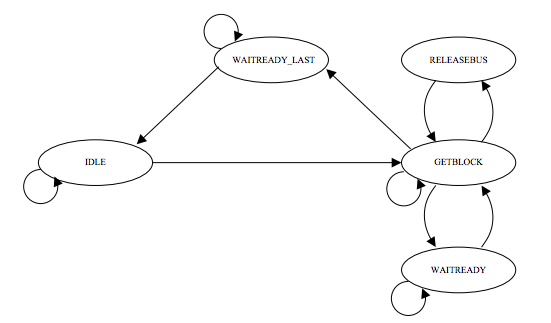
\includegraphics[width=280px]{fsmlab3.png}
\caption{Tillståndsgraf för vår utökade design}
\label{fig:state}
\end{figure}
För att lösa uppgiften så implementerade vi tillståndsgrafen i figur \ref{fig:state2} ganska rakt av med hjälp av en DMA. Maskinen börjar i \lq\lq{}Idle\rq\rq{}, får en startsignal och börjar hämta block med 8x8 pixlar från minnet, skickar iväg pixlarna till acceleratorn och inväntar sedan en signal att den är färdig. Då hämtar den ett nytt block och håller på så tills hela bilden är bearbetad. \lq\lq{}Releasebus\rq\rq{} är till för att då och då släppa bussen så att någon annan i maskinen kan få skicka saker via bussen, annars hade DMA\rq{}n tagit beslag på bussen väldigt länge och inget annat skulle hända i datorn medans DMA\rq{}n hämtade data.

\begin{figure}[h]
\centering
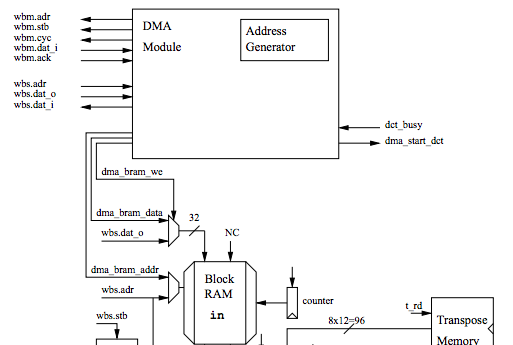
\includegraphics[width=280px]{architecturelab3.png}
\caption{Arkitektur för vår utökade design}
\label{fig:arch3}
\end{figure}
Figur \ref{fig:arch3} visar hur DMA\rq{}n är kopplad till acceleratorn och hur den kontrollerar vilka signaler som kommer in, antingen från bussen eller från DMA\rq{}n. Jämför med figur \ref{fig:architecture} för att se resten av designen. I DMA modulen finns bara register för att hålla koll på vilket tillstånd maskinen befinner sig i, när vissa villkor är uppfyllda byts tillståndet och korrekta åtgärder vidtas. En räknare håller koll på hur många pixlar som har lästs in, när det har lästs 4 pixlar skickas de till acceleratorn, \lq\lq{}Waitready\rq\rq{}. Detta görs om och om igen tills hela bilden är färdig då vi istället går till \lq\lq{}Waitreadylast\rq\rq{} och sedan tillbaka till \lq\lq{}Idle\rq\rq{}.

Verifiering av hårdvaran skedde genom att köra de tidigare testerna i modelsim och när rätt signaler lades på så testade vi att konvertera en raw fil till jpeg vilket fungerade. Mjukvaran som kallade på DMA\rq{}n skickade en startsignal och väntade sedan på att acceleratorn skulle sätta färdigbiten i dess statusregister, därefter läste mjukvaran av utminnet och skickade en fortsätt-signal, detta skedde tills bilden var klar. 

Det som skickas på bussen är således en startsignal från mjukvaran, 8x8 pixlar till DMA\rq{}n, varpå mjukvaran kontinuerligt läser av statusregistret för att se när blocket är färdigt, varpå mjukvaran kan läsa av de 8x8 pixlarna. All den kommunikationen görs tills bilden är färdig.

\section{Resultat}

\subsection{Prestanda}

\begin{table}[H]
    \centering
    \begin{tabular}{l l}
    
        Beskrivning & Antal klockcykler\\
        \hline
        Main program  & 33 902 171 \\
        Init  &  9 850 924 \\
        Encode\_image  & 24 051 247 \\
        Forward\_DCT  & 8 317 191 \\
        Copy  & 1 518 825 \\
        DCT kernel  & 0 \\
        Quantization  & 6 798 366 \\
        Huffman encoding  & 15 246 407 \\
        Emit\_bits  & 7 904 811 \\
    \end{tabular}
    \caption{ Prestanda för JPEG-acceleratorn }
    \label{tab:jpeg_performance_2}
\end{table}
\begin{table}[H]
    \centering
    \begin{tabular}{l l}
    
        Beskrivning & Antal klockcykler\\
        \hline
        Main program  & 25 847 242 \\
        Init  & 6 600 044 \\
        Encode\_image  & 19 247 198 \\
        Forward\_DCT  & 6 489 189 \\
        Copy  & 0 \\
        DCT kernel  & 0 \\
        Quantization  & 6 489 189 \\
        Huffman encoding  & 12 226 950 \\
        Emit\_bits  & 4 983 905 \\
    \end{tabular}
    \caption{ Prestanda för JPEG-acceleratorn med inkopplad DMA }
    \label{tab:jpeg_performance_3}
\end{table}

Tabell \ref{tab:jpeg_performance_2} visar prestandan för labb2 och tabell \ref{tab:jpeg_performance_3} för labb3, i \lq\lq{}Copy\rq\rq{} har prestandan sjunkit med 1,5 miljoner klockcykler! Totalt gick labb3 8 miljoner klockcykler.

\subsection{FPGA-användning}
\begin{table}[H]
    \centering
    \begin{tabular}{l l l}
        Flip Flops   &      7 273 out of   46080  & 15\% \\
        4 input LUTs &      11 485 out of  46080  & 24\% \\
        MULT18X18s   &      19 out of 120  &   15\% \\
        RAMB16s      &      42 out of 120  &   35\% \\
    \end{tabular}
    \caption{ De mest intressanta delarna ur syntes-rapporten för JPEG-acceleratorn utan DMA. }
    \label{tab:fpga_usage2}
\end{table}
\begin{table}[H]
    \centering
    \begin{tabular}{l l l}
        Flip Flops   &      7 408 out of   46080  & 16\% \\
        4 input LUTs &      11 986 out of  46080  & 26\% \\
        MULT18X18s   &      19 out of 120  &   15\% \\
        RAMB16s      &      42 out of 120  &   35\% \\
    \end{tabular}
    \caption{ De mest intressanta delarna ur syntes-rapporten för JPEG-acceleratorn med DMA. }
    \label{tab:fpga_usage3}
\end{table}

Tabell \ref{tab:fpga_usage2} visar en del ur syntetiseringsrapporten för acceleratorn, jämför man med tabell \ref{tab:fpga_usage3} så ser man att DMA\rq{}n inte gav så stor skillnad i storlek, men gav bra prestandaförbättring så det var värt att implementera den.

\section{Filer}
\begin{itemize}
        \item [jpegtop.sv] Mestadels av designen skedde här, våra kontrollsignaler ligger här tillsammans med flera räknare och minnen.
        \item [transpose.sv] Transponeringsminnet fick en egen fil med en kolumnräknare och en radräknare för att hålla koll på vart grunkan håller på att läsa respektive skriva.
        \item [q2.sv] Denna sköter multipliceringen med reciprokalerna och skickar sedan resultatet till utminnet.
        \item [jpegdma.sv] Designen för den andra biten där jpeg-acceleratorn själv läser av informationen i minnet.
\end{itemize}


\newpage
\begin{appendices}
\begin{changemargin}{-3cm}{-3cm} 
\section{jpegtop.sv}
\lstinputlisting[language=Verilog,caption={Kod för labb 2},label=jpeg_top]{jpeg_top.sv}

\section{transpose.sv}
\lstinputlisting[language=Verilog,caption={Kod för transponeringen},label=selection-sort]{transpose.sv}

\section{Q2.sv}
\lstinputlisting[language=Verilog,caption={Kod för kvantiseringen},label=q2]{q2.sv}

\section{jpegdma.sv}
\lstinputlisting[language=Verilog,caption={Kod för labb 3},label=jpeg_dma]{jpeg_dma.sv}
\end{changemargin}
\end{appendices}


\end{document}